% DO NOT COMPILE THIS FILE DIRECTLY!
% This is included by the other .tex files.

\begin{frame}
\titlepage
\end{frame}

\begin{frame}
  \frametitle{The aim of this presentation}
  \begin{itemize}
     \item What has happened since the 2021 MISP summit
     \item Give you a brief update over the highlights from the past year
     \item Upcoming changes
  \end{itemize}
\end{frame}

\begin{frame}
  \frametitle{MISP's evolution since the last MISP summit}
  \begin{itemize}
    \item Since the last MISP summit (09/2021) we've had:
    \begin{itemize}
        \item {\bf 16} releases
        \item {\bf 3768} commits
        \item {\bf 100} contributors contributing to the core software and its components
    \end{itemize}
  \end{itemize}
\end{frame}

\begin{frame}
  \frametitle{A topical listing of the new major features}
  \begin{itemize}
      \item Internals and core feature improvements
      \item Integrations
      \item Security
  \end{itemize}
\end{frame}

\begin{frame}
  \frametitle{Internals and core feature improvements}
\end{frame}

\begin{frame}
  \frametitle{Continuous work on preparing a tech stack switch}
  \begin{itemize}
      \item {\bf Refactoring} the code base
      \item Fixing several long standing issues
      \item Heavy focus also on {\bf integration}
      \item {\bf Documentation} of existing functionalities and mappings
      \item Building on and reusing {\bf Cerebrate's codebase}
  \end{itemize}
\end{frame}

\begin{frame}
\frametitle{New background processing library}
\begin{itemize}
	\item Finally, it is time to sunset the ancient background processor of MISP
        \item New tool, built from the ground up by Luciano Righetti
        \begin{itemize}
            \item More simplistic, relying on {\bf Supervisord}
            \item No bloated scheduling - reliance on {\bf cron jobs}
            \item Internally {\bf compatible} with the old processor
        \end{itemize}
        \item For a period of time we will be {\bf supporting both} concurrently
\end{itemize}
\end{frame}

\begin{frame}
  \frametitle{Sharing group blueprints}
  \begin{itemize}
     \item Solving the issue of {\bf sharing group lifecycle management}
     \item Build SG blueprints for reusable, maintainable sharing groups
     \item Abstract sharing groups, organisation metadata as building blocks
     \item Solve newly arising sharing challenges
  \end{itemize}
\end{frame}

\begin{frame}
\frametitle{Sharing group blueprints}
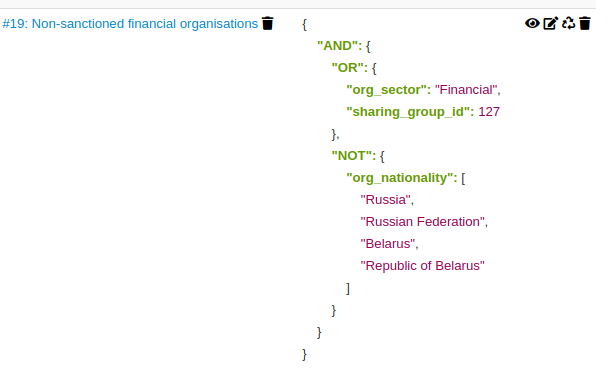
\includegraphics[scale=0.6]{images/blueprints2.png}
\end{frame}

\begin{frame}
  \frametitle{Further synchronisation filtering methods}
  \begin{itemize}
     \item The ability to {\bf exclude} certain attribute {\bf types from the synchronisation}
     \item Comes with some risks, but solves some issues
     \item An example: {\bf Exclusion of malware samples when sharing towards classified networks}
  \end{itemize}
\end{frame}

\begin{frame}
  \frametitle{Advanced timelining}
  \begin{itemize}
     \item Rework of the timelining in MISP
     \item Inclusion of images, sightings
     \item Various other improvements
  \end{itemize}
\end{frame}

\begin{frame}
\frametitle{Timelining}
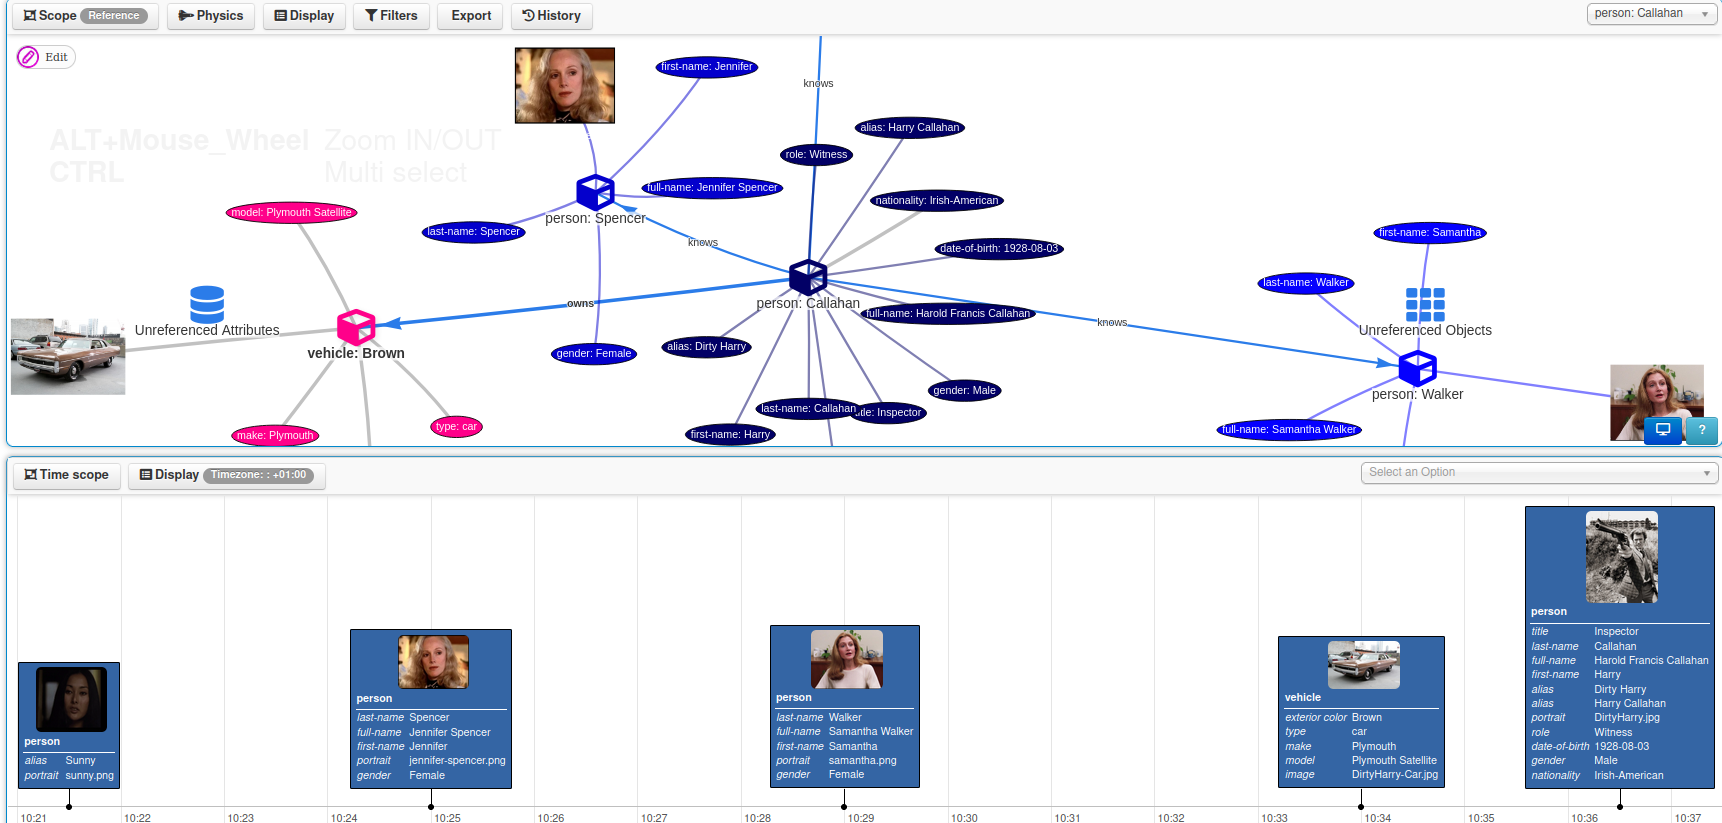
\includegraphics[scale=0.2]{images/timelining.png}
\end{frame}

\begin{frame}
  \frametitle{Periodic notifications}
  \begin{itemize}
     \item Optional {\bf digest based notifications} rather than publish alerts
     \item Inclusion of images, sightings
     \item Various other improvements
  \end{itemize}
\end{frame}

\begin{frame}
\frametitle{Periodic notifications}
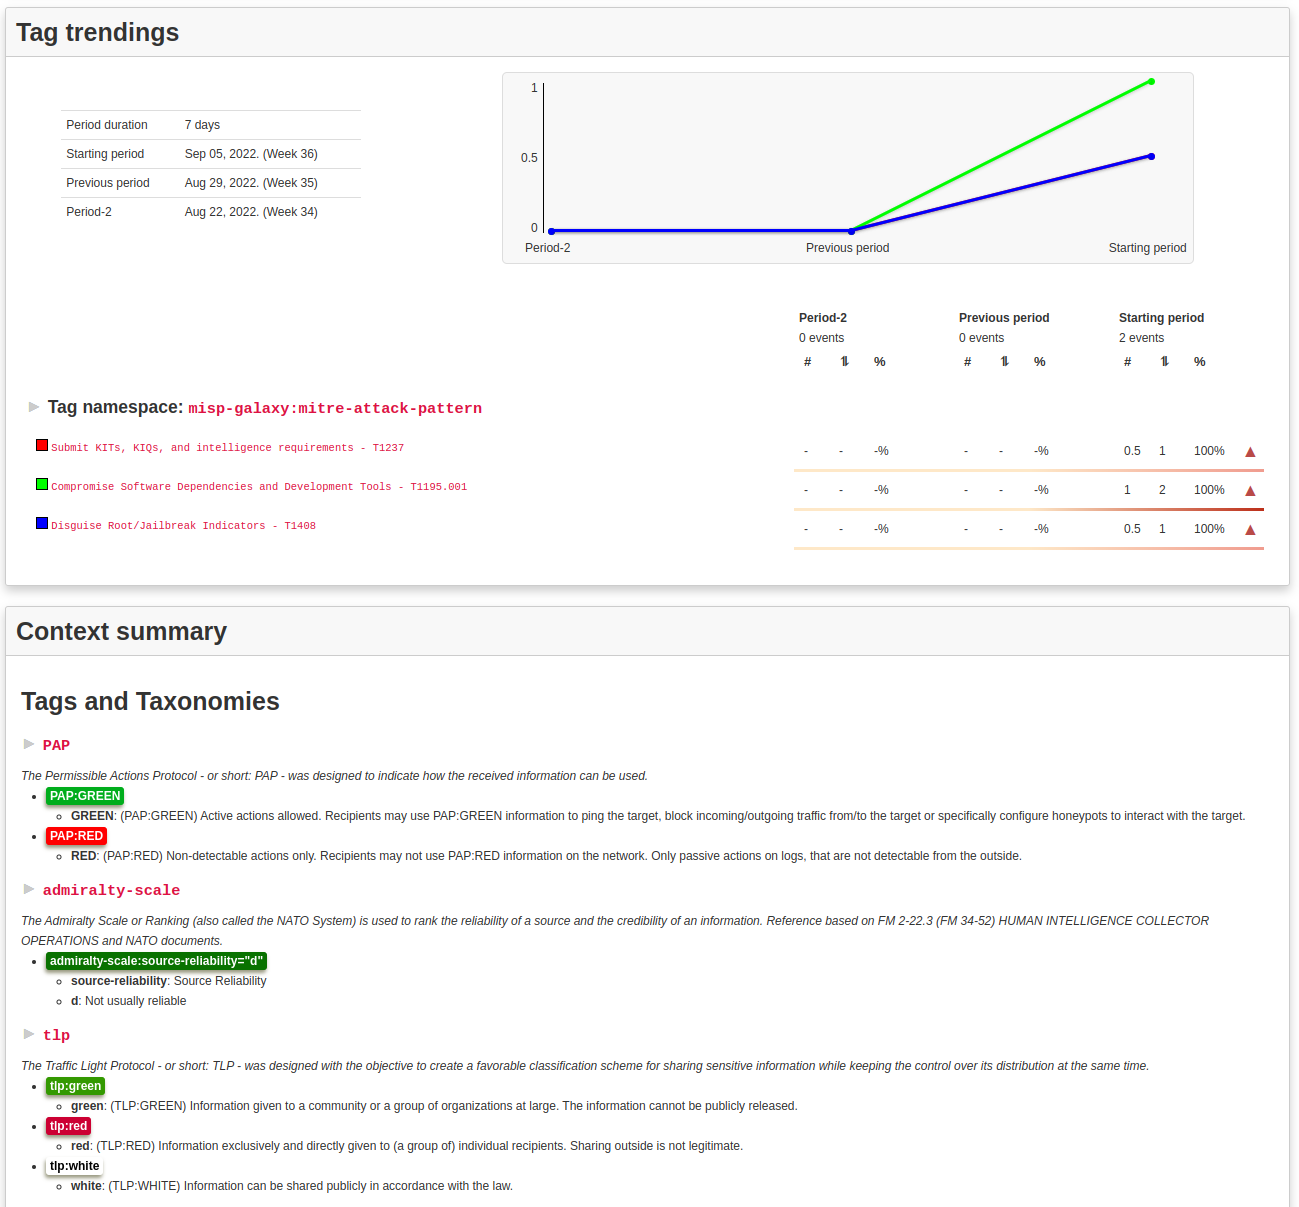
\includegraphics[scale=0.2]{images/periodic.png}
\end{frame}

\begin{frame}
  \frametitle{New correlation engine}
  \begin{itemize}
     \item Massive {\bf performance bump} and storage size decrease
     \item Automatic {\bf overcorrelation protection}
     \item {\bf No ACL} mode for {\bf endpoint MISPs}
     \item Extensible system for future, alternate engines
  \end{itemize}
\end{frame}

\begin{frame}
  \frametitle{Custom E-mail templates}
  \begin{itemize}
     \item Build text/HTML templates for {\bf custom publish alerts}
     \item Drop the templates in the appropriate directory and you're good to go
     \item Enrollment and password reset templates also supported
  \end{itemize}
\end{frame}

\begin{frame}
  \frametitle{Continuous improvements}
  \begin{itemize}
      \item Massive list of {\bf quality of life} improvements
      \item {\bf Performance} fixes
      \item Loads of nice new improvements for you to discover
      \item Massive shoutout to the hero of fixing the mess we've made: {\bf Jakub Onderka}
  \end{itemize}
\end{frame}


\begin{frame}
  \frametitle{Integrations}
\end{frame}

\begin{frame}
  \frametitle{OpenAPI}
  \begin{itemize}
     \item Full documentation of our APIs by Luciano Righetti
     \item {\bf New API pages}
     \item Sample {\bf payloads, descriptions, expected responses}
     \item Makes integrating / using the API a breeze
  \end{itemize}
\end{frame}

\begin{frame}
\frametitle{OpenAPI}
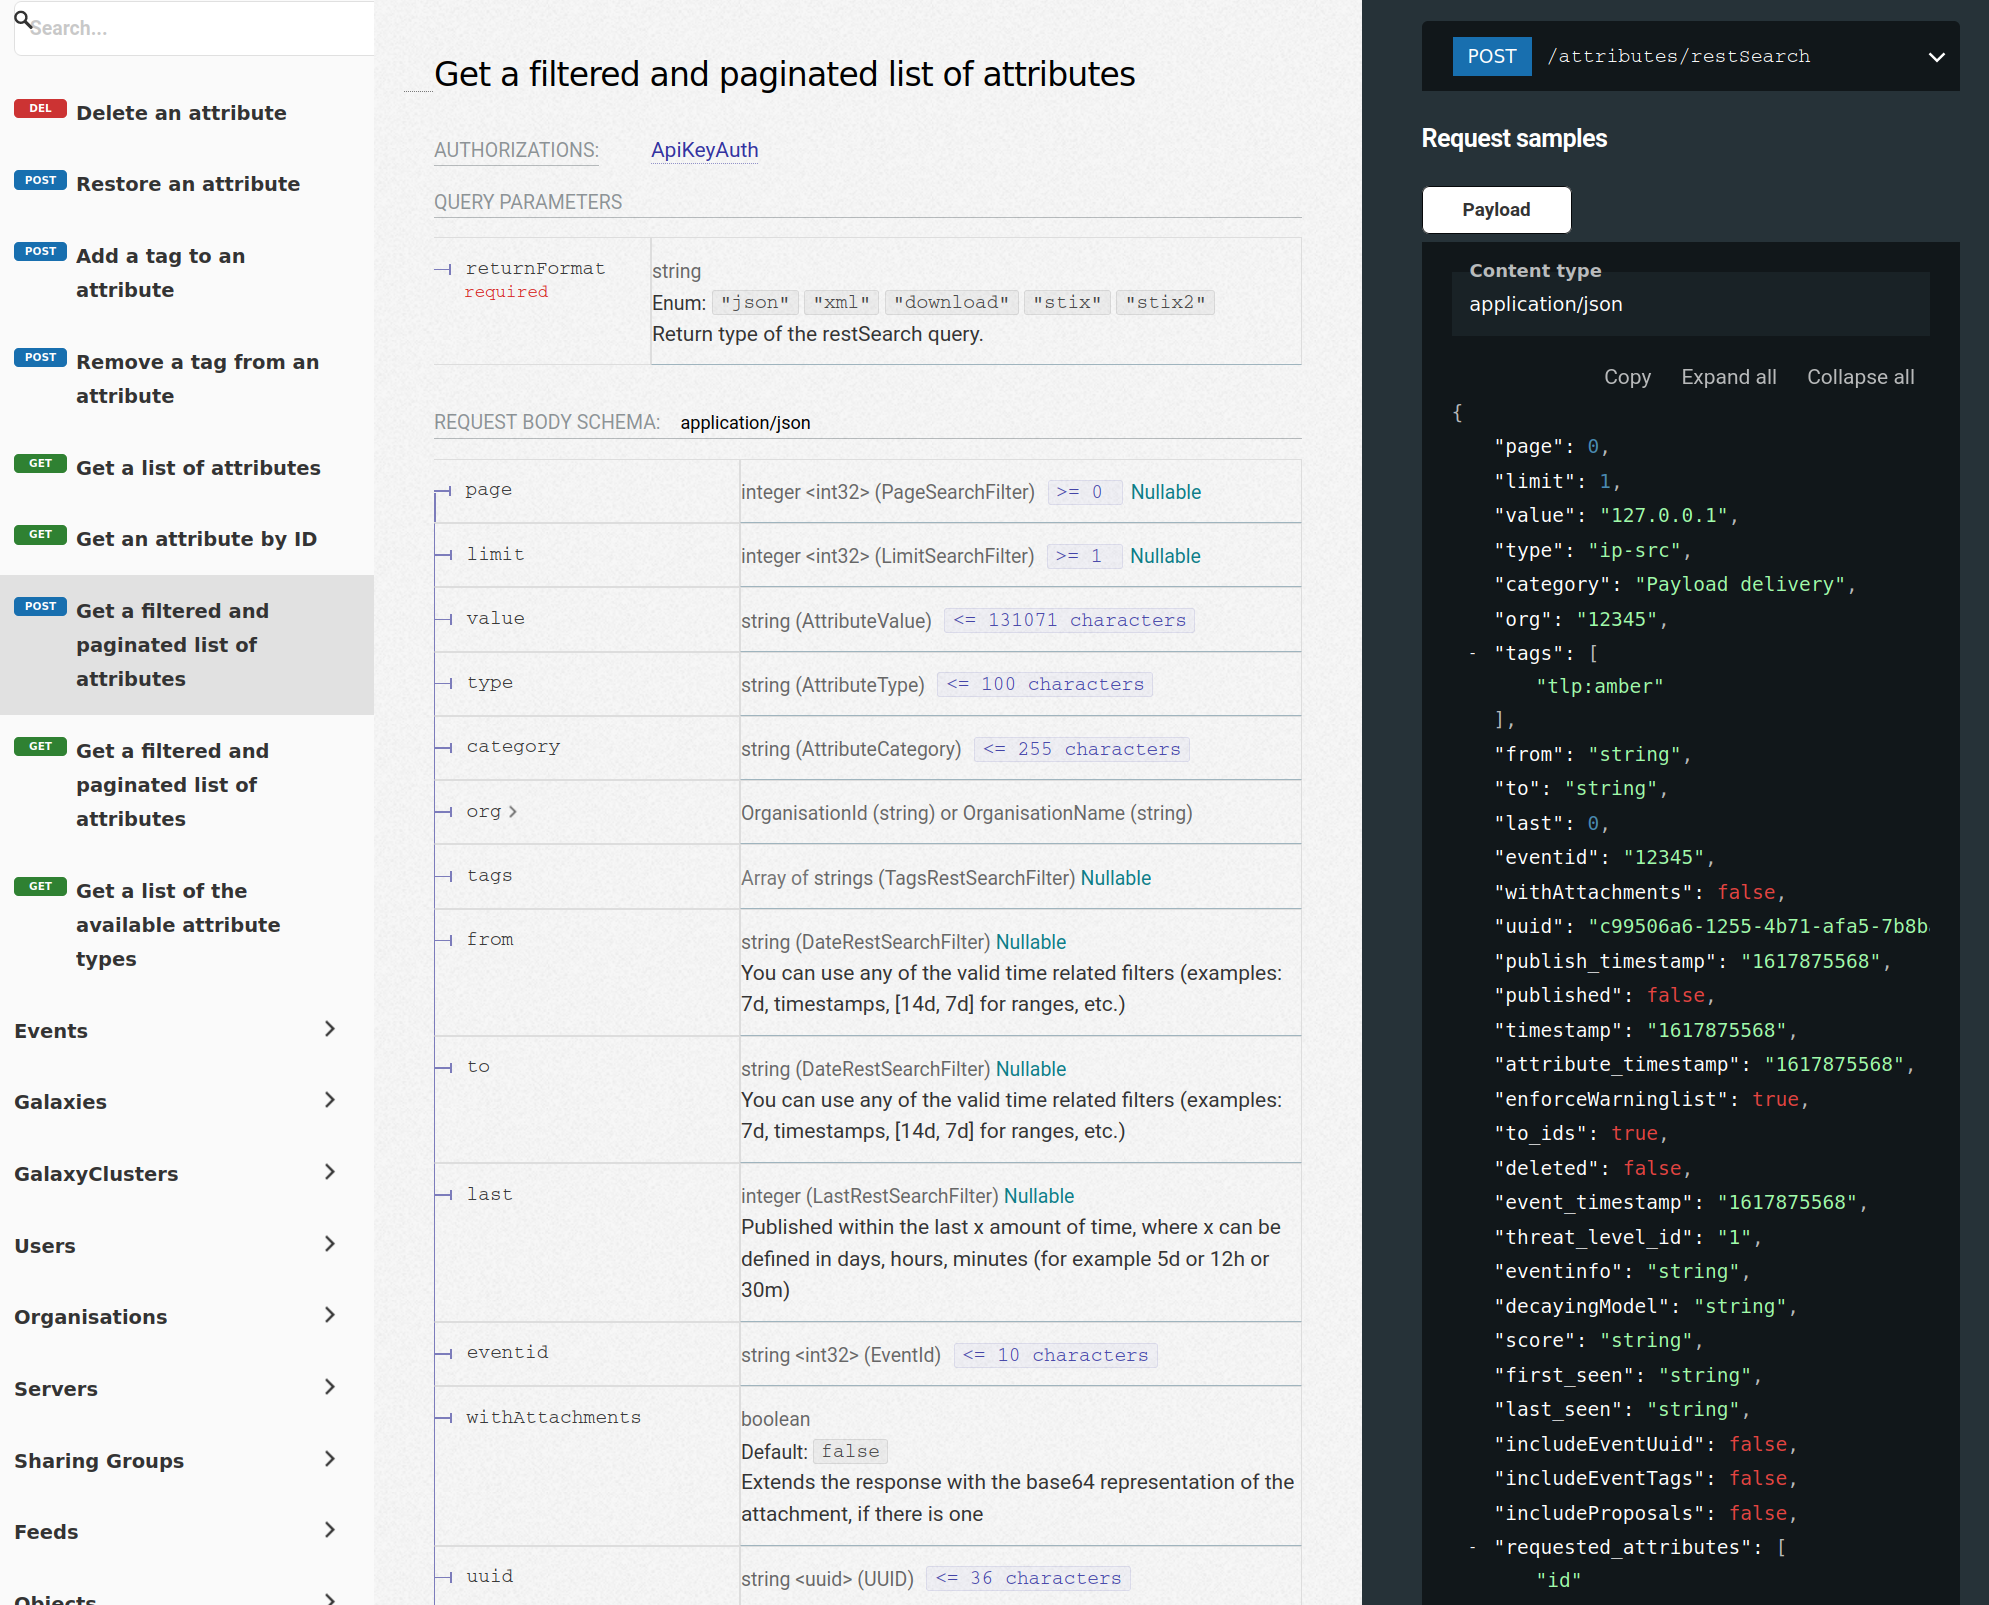
\includegraphics[scale=0.15]{images/openapi_page.png}
\end{frame}

\begin{frame}
  \frametitle{Workflows}
  \begin{itemize}
     \item Brief recap, as presented earlier today by Sami
     \item Modify {\bf existing execution paths}
     \item Bake in {\bf interactions with other tools}
     \item Build extensive {\bf decision trees}
  \end{itemize}
\end{frame}

\begin{frame}
\frametitle{Workflows}
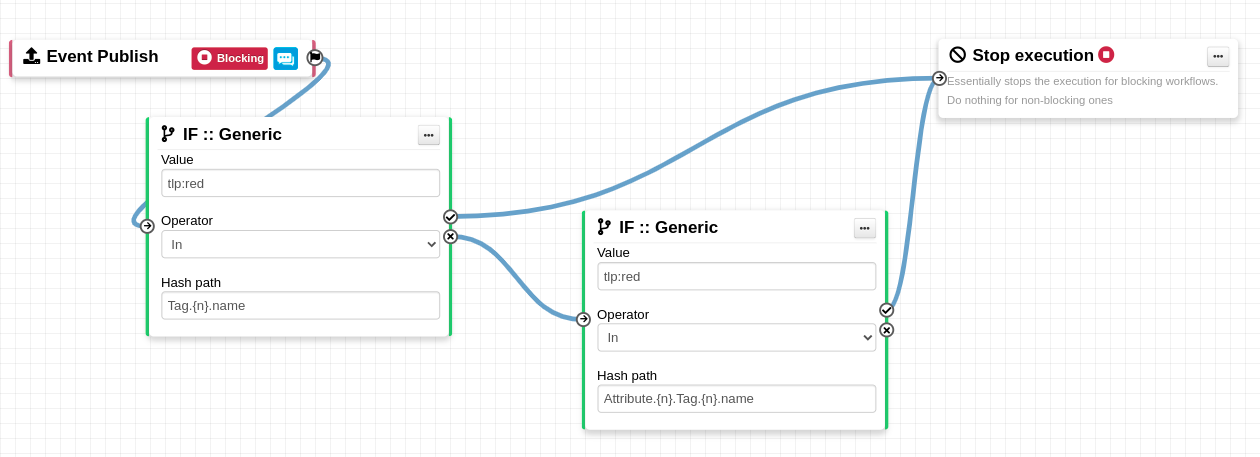
\includegraphics[scale=0.25]{images/workflows.png}
\end{frame}

\begin{frame}
  \frametitle{STIX libraries}
  \begin{itemize}
     \item {\bf Massive rework}, the outcome of over a year of development by Christian Studer
     \item Added STIX 2.1 support on export
     \item STIX 1.1.1, 1.2, 2.0, {\bf 2.1} all supported
     \item Much more complex, in-depth mapping, aiming for {\bf 100\% coverage of the standard}
     \item Collaboration with {\bf DHS and MITRE}
     \item The MISP->STIX converters became their own {\bf standalone library}
     \item Extensive {\bf documentation} and examples for all possible generated objects
     \item Test suites to validate against MITRE's libraries
     \item {\bf For a deep dive, make sure to catch Christian's talk tomorrow!}
  \end{itemize}
\end{frame}

\begin{frame}
\frametitle{OpenAPI}
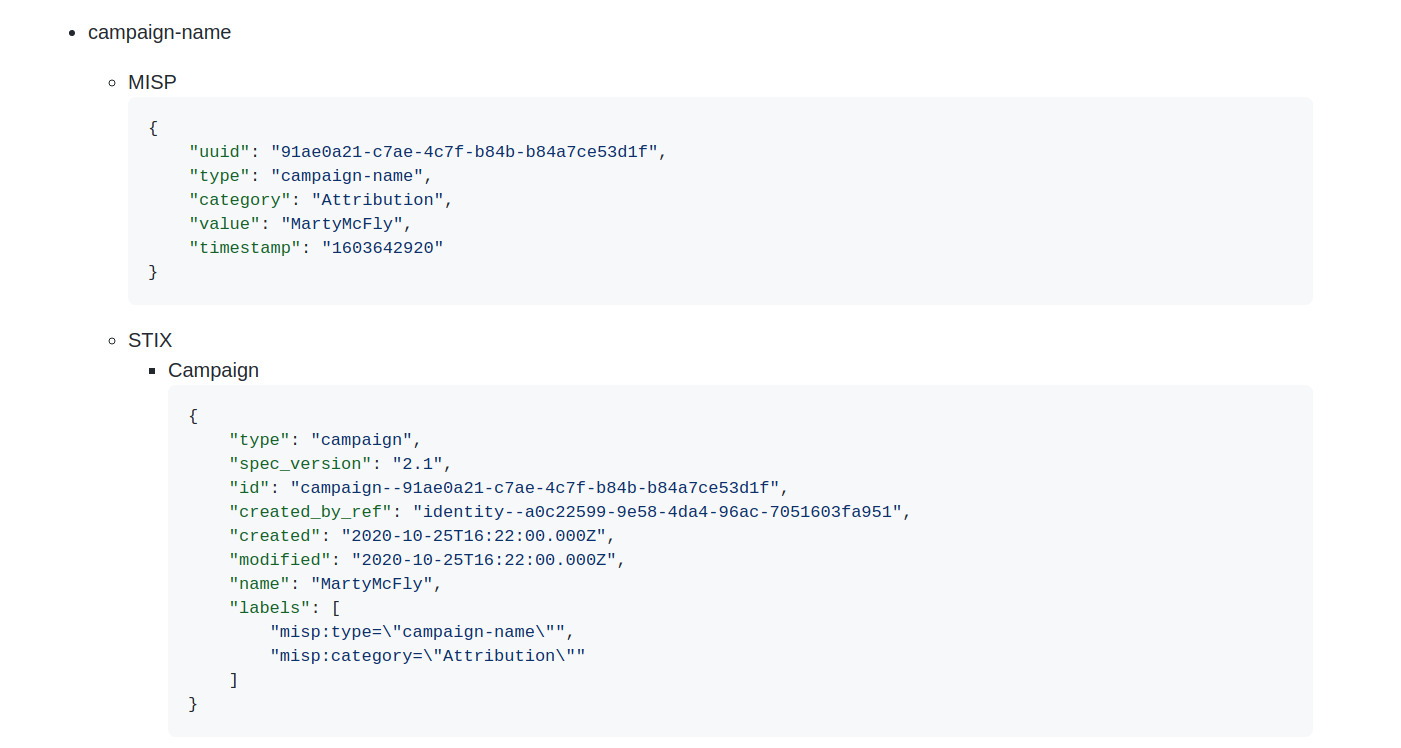
\includegraphics[scale=0.4]{images/stix.png}
\end{frame}

\begin{frame}
  \frametitle{Cerebrate integration}
  \begin{center}
  
\includegraphics[scale=0.1]{images/cerebrate-logo.png}
  \end{center}
  \begin{itemize}
     \item Cerebrate session tomorrow
     \item Integration with the {\bf contact management} system
     \item Functionalities to allow {\bf management by Cerebrate}
  \end{itemize}
\end{frame}

\begin{frame}
\frametitle{mail2misp 1.0 release}
\begin{itemize}
	\item A tool we've been using internally for a long time
        \item First official release
        \item {\bf Receive, parse, encode} emails as MISP events
        \item Works with existing mail infrastructure or via a spamtrap
        \item Configure extensive {\bf parsing rules}
        \item Built and maintained by our colleague Sascha Rommelfangen
\end{itemize}
\end{frame}

\begin{frame}
\frametitle{Integrations}
\begin{itemize}
	\item New MISP modules and improvements to existing ones
        \item Some examples:
        \begin{itemize}
            \item Integration with Alexandre Dulaunoy's new Hashlookup service
            \item Passive SSH integration
            \item Recorded Future module
        \end{itemize}
\end{itemize}
\end{frame}


\begin{frame}
  \frametitle{Security}
\end{frame}


\begin{frame}
  \frametitle{Cryptographic signing and tamper protection}
  \begin{itemize}
     \item Need to be able to share and ensure the {\bf veracity of critical events}
     \item Tampering by {\bf malicious intermediaries}, even in closed networks became a new fear
     \item We came up with a solution that allows us to {\bf lock down critical events}
     \item Limits the distribution, but {\bf increases the resilience} of MISP immensely
  \end{itemize}
\end{frame}

\begin{frame}
\frametitle{Cryptographic signing and tamper protection}
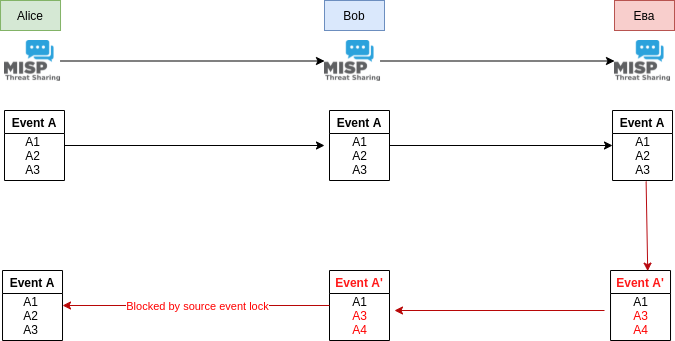
\includegraphics[scale=0.5]{images/signing1.png}
\end{frame}

\begin{frame}
\frametitle{Cryptographic signing and tamper protection}
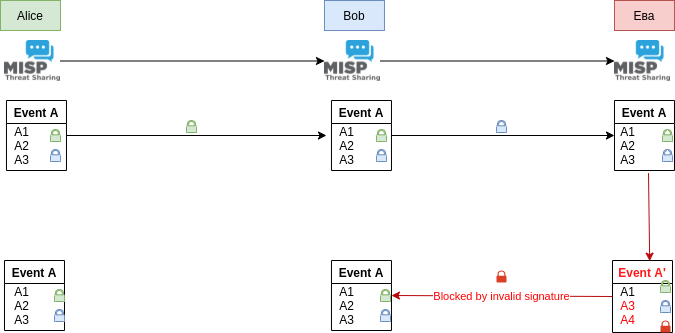
\includegraphics[scale=0.5]{images/signing2.png}
\end{frame}

\begin{frame}
\frametitle{Cryptographic signing and tamper protection}
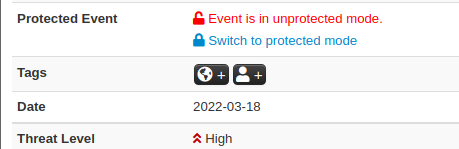
\includegraphics[scale=0.6]{images/signing3.png}
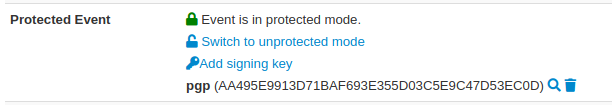
\includegraphics[scale=0.6]{images/signing4.png}
\end{frame}

\begin{frame}
  \frametitle{Security fixes}
  \begin{itemize}
     \item Long list of penetration test results shared with us by the community...
     \item ...including an in-depth series conducted by {\bf Zigrin security on behalf of the Luxembourgish army}
     \item 11 new CVEs in the past year
     \item Long list of usability/bug fixes as a secondary outcome of the pentest reports
  \end{itemize}
\end{frame}

\begin{frame}
  \frametitle{The Future}
  \begin{itemize}
     \item Stack switch to Cerebrate's codebase
     \item Many new systems that have are built to be fleshed out
     \begin{itemize}
         \item {\bf Workflows} - new hooks, inter-module interactions, sample blueprints
         \item Custom {\bf correlation engines}
         \item Tighter integration with {\bf Cerebrate}
         \item {\bf Cryptographic securing} of exchanges
     \end{itemize}
     \item Continuous improvements to integrations
     \begin{itemize}
         \item New {\bf modules}, improving existing ones
         \item Tighter integration with {\bf STIX/TAXII}
         \item Refinement of the {\bf APIs} and supporting libraries
     \end{itemize}
     \item Tighter integration with {\bf IAM} systems
     \item Sanity checking our list of deprecated functionalities
  \end{itemize}
\end{frame}

\begin{frame}
  \frametitle{To sum it all up...}
  \begin{itemize}
     \item The MISP {\bf developer community} continues to grow and stay active
     \item The main focus the past year was on the following
     \begin{itemize}
          \item Performance, security, UX improvements
          \item Customisations of workflow processes
          \item Better operationalisation of MISP (community management, integration, monitoring)
          \item Fleshing out the documentation and supporting materials
     \end{itemize}
     \item Cerebrate is aiming to fill the void of community/fleet management that we currently have
     \item Definitely no lack of new ideas and improvements, if you want to participate, it's easy to {\bf get involved}
     \item Prioritisation is hard. {\bf Let us know what you think we should focus on}!
  \end{itemize}
\end{frame}

\begin{frame}
  \frametitle{Get in touch if you have any questions}
  \begin{itemize}
    \item Contact CIRCL
    \begin{itemize}
      \item info@circl.lu
      \item \url{https://twitter.com/circl_lu}
      \item \url{https://www.circl.lu/}
    \end{itemize}
    \item Contact MISPProject 
    \begin{itemize}
      \item \url{https://github.com/MISP}
      \item \url{https://gitter.im/MISP/MISP}
      \item \url{https://twitter.com/MISPProject}
    \end{itemize}
    \item Cerebrate project
    \begin{itemize}
      \item \url{https://github.com/cerebrate-project}
      \item \url{https://github.com/cerebrate-project/cerebrate}
    \end{itemize}
  \end{itemize}
\end{frame}
